\section{Current Sensing}
An important requirement set by the lead of the project was that we sense the current drawn by the BLDC motor. We choose for a `INA181A3QDBVRQ1`. this is an Automotive, Bidirectional, Low- and High-Side Voltage Output,
Current-Sense Amplifiers which needs a shunt resistor. Current sense resistors, or shunt resistors, are devices used to gauge the flow of current. They detect and convert current to a measured output voltage. Current sense resistors are generally low-value, high-power resistors. The IC will sent out an value which will be read buy the ADC of the STM32. 
\begin{figure}[H]
    \centering
    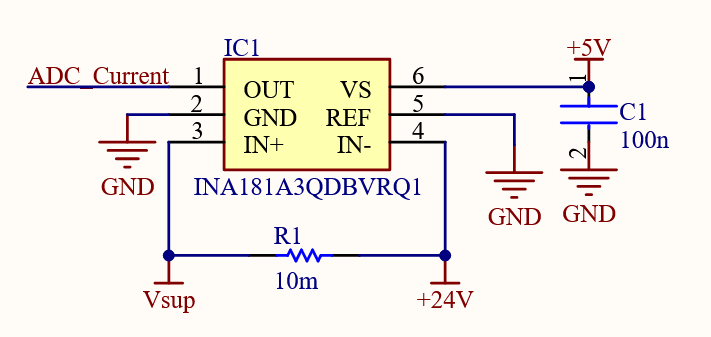
\includegraphics[width=0.5\linewidth]{img/Currentsense schem.png}
    \caption{Current sensing}
    \label{fig:Current sense Schem}
\end{figure}

Although this circuit may appear intriguing and effective, there is room for improvement. We opted for a different IC, the INA236BIDDFR, which is a 16-bit, Ultra-Precise Current, Voltage, and Power Monitor with an I\textsuperscript{2}C interface. This means that instead of utilizing the 12-bit ADC from the STM32F411, we now employ the 16-bit ADC from the INA236, allowing for \(2^{16}-2^{12}=61440\) additional data points, significantly enhancing accuracy. 
\begin{table}[H]
\begin{tabular}{|c|c|}
\hline
\rowcolor[HTML]{C0C0C0} 
\textbf{A0} & \textbf{INA236B DEVICE OPTION} \\ \hline
GND         & 1001000                        \\ \hline
VS          & 1001001                        \\ \hline
SDA         & 1001010                        \\ \hline
SCL         & 1001011                        \\ \hline
\end{tabular}
\end{table}
Furthermore, the measured values are transmitted via I\textsuperscript{2}C, providing flexibility in selecting the device address. We selected address 1001000 by connecting the \textbf{REF} to to \textbf{GND}, as it was available and not in use by our Raspberry Pi or Display.

